\documentclass[border=4pt]{standalone}
\usepackage{amsmath,amssymb}
\usepackage{tikz}
\usetikzlibrary{shapes,arrows.meta,positioning}

\begin{document}
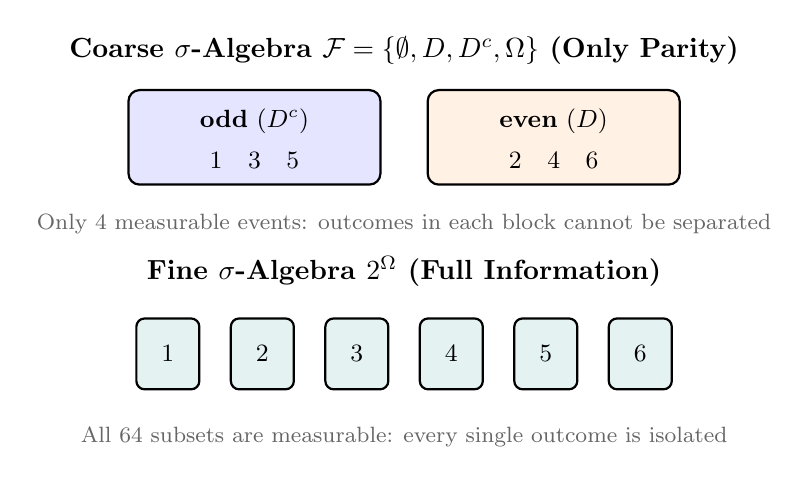
\begin{tikzpicture}[font=\small]
  % Case A: Parity
  \node[font=\bfseries] at (3.5, 3.2) {Coarse $\sigma$-Algebra $\mathcal{F} = \{\emptyset, D, D^c, \Omega\}$ (Only Parity)};
  \draw[thick, fill=blue!10, rounded corners=4pt] (0,1.5) rectangle (3.2, 2.7);
  \node at (1.6, 2.3) {\textbf{odd} ($D^c$)};
  \node at (1.6, 1.8) {$1 \quad 3 \quad 5$};

  \draw[thick, fill=orange!10, rounded corners=4pt] (3.8,1.5) rectangle (7.0, 2.7);
  \node at (5.4, 2.3) {\textbf{even} ($D$)};
  \node at (5.4, 1.8) {$2 \quad 4 \quad 6$};
  
  \node[align=center, font=\footnotesize, text=gray!80!black] at (3.5, 1.0) {Only 4 measurable events: outcomes in each block cannot be separated};

  % Case B: Power set
  \begin{scope}[yshift=-2.8cm]
    \node[font=\bfseries] at (3.5, 3.2) {Fine $\sigma$-Algebra $2^\Omega$ (Full Information)};
    \foreach \x/\val in {0.5/1, 1.7/2, 2.9/3, 4.1/4, 5.3/5, 6.5/6} {
      \draw[thick, fill=teal!10, rounded corners=3pt] (\x-0.4, 1.7) rectangle (\x+0.4, 2.6);
      \node at (\x, 2.15) {$\val$};
    }
    \node[align=center, font=\footnotesize, text=gray!80!black] at (3.5, 1.1) {All 64 subsets are measurable: every single outcome is isolated};
  \end{scope}
\end{tikzpicture}
\end{document}
